\documentclass[twocolumn]{article}
\usepackage{amsmath, amssymb, amsthm}
\usepackage{tikz}
\usetikzlibrary{arrows,decorations.markings}
\usetikzlibrary{calc}
\usetikzlibrary{patterns}
\usepackage{pgfplots}
\usepgflibrary{patterns}
\usepackage[T1]{fontenc}
\usepackage{mathptmx}
\usepackage{halloweenmath}
\usepackage{textcomp}
%\usepackage{simpsons}
\usepackage{multicol}
\usepackage{makecell}
\usepackage[makeroom]{cancel}
\usepackage{lscape}
\usepackage[utf8]{inputenc}
\usepackage{pdfpages}
\usepackage{geometry}
 \geometry{
	 a4paper,
	 left=10mm,
	 right=10mm,
	 top=10mm,
	 bottom=20mm,
	 }
\usepackage{hyperref}
\begin{document}
\newcommand{\thicc}{thick}
\Large
\begin{equation*}
	\frac{d}{dt}\Bigg{\{} U + m \Bigg{(}\frac{c^2}{2}+gz\Bigg{)}\Bigg{\}} 
	= 
	\sum_{j}{\Bigg{[}\dot{m}_j\Bigg{(}h+\frac{c^2}{2}+gz\Bigg{)}_j \Bigg{]}}  
	+ 
	\sum_{l}^{} \Big(\dot{Q}_t\Big)_l 
	+ 
	\sum_{i}\Big(\dot{W}_t\Big)_i
	-
	p\frac{dV}{dt}
\end{equation*}

\normalsize

%    _   __                           __   __      __            
%   / | / /___  ____ ___  ___  ____  / /__/ /___ _/ /___  _______
%  /  |/ / __ \/ __ `__ \/ _ \/ __ \/ //_/ / __ `/ __/ / / / ___/
% / /|  / /_/ / / / / / /  __/ / / / ,< / / /_/ / /_/ /_/ / /    
%/_/ |_/\____/_/ /_/ /_/\___/_/ /_/_/|_/_/\__,_/\__/\__,_/_/     

\section{Nomenklatur}


\begin{align*}
	\mathbf{An}		&=	\text{Anergie[J]} \\
	\mathbf{c_s}		&=	\text{Schallgeschwindigkeit[m/s]} \\
	\mathbf{c_p}		&=	\text{Spezifische Wärmekapazität dp = 0 [J/kg*K]} \\
	\mathbf{c_v}		&=	\text{Spezifische Wärmekapazität dv = 0 [J/kg*K]} \\
	\mathbf{E}		&=	\text{Energie[J]} \\
	\mathbf{Ex = -W_{ex}}	&=	\text{Exergie[J]} \\
	\mathbf{F}		&=	\text{Kraft[N]} \\
	\mathbf{F = U - TS}	&=	\text{Freie Energie[J]} \\
	\mathbf{f = u-Ts}	&=	\text{Spezifische freie Energie[J/kg]} \\
	\mathbf{f}		&=	\text{Fugazität[Pa]} \\
	\mathbf{G = H -TS}	&=	\text{Freie Enthalpie[J]} \\
	\mathbf{g = h -Ts}	&=	\text{Spezifische freie Enthalpie[J/kg]} \\
	\mathbf{g}		&=	\text{Erdbeschleunigung[m/s²]} \\
	\mathbf{H = U+pV}	&=	\text{Enthalpie[J]} \\
	\mathbf{h = u + pv}	&=	\text{Spezifische Enthalpie[J/kg]} \\
	\mathbf{\Delta Hg}	&=	\text{Molare Reaktionsenthalpie} \\
	\mathbf{K}		&=	\text{Konstante des Massenwirkungsgesetztes[-]} \\
	\mathbf{M}		&=	\text{Molmasse[kg/mol]} \\
	\mathbf{\dot{m}}	&=	\text{Massestrom[kg/s]} \\
	\mathbf{m'}		&=	\text{Masse in der flüssigen Phase[kg]} \\
	\mathbf{m''}		&=	\text{Masse in der gasförmigen Phase[kg]} \\
	\mathbf{Ma=c/c_s}	&=	\text{Machzahl[-]} \\
	\mathbf{n=m/M}		&=	\text{Molzahl[mol]} \\
	\mathbf{n}		&=	\text{Polytropenexponent[-]} \\
	\mathbf{P_t}		&=	\text{technische Leistung[W]} \\
	\mathbf{Q}		&=	\text{Wärme[J]} \\
	\mathbf{\dot{Q}}	&=	\text{Wärmestrom[W]} \\
	\mathbf{q}		&=	\text{Spezifische Wärme[J/kg]} \\
	\mathbf{r}		&=	\text{Spezifische Verdampfungsenthalpie[J/kg]} \\
	\mathbf{R}		&=	\text{Gaskonstante[J/(kg K)]} \\
	\mathbf{R_m}		&=	\text{Universelle Gaskonstante[J/(mol K)]} \\
	\mathbf{S}		&=	\text{Entropie[J/K]} \\
	\mathbf{s}		&=	\text{Spezifische Entropie[J/(kg K)]} \\
	\mathbf{T}		&=	\text{Temperatur[K]} \\
	\mathbf{t}		&=	\text{Zeit[s]} \\
	\mathbf{t}		&=	\text{Temperatur[\textcelsius{}]} \\
	\mathbf{T}		&=	\text{Sättigungstemperatur[K]} \\
	\mathbf{U}		&=	\text{Innere Energie[J]} \\
	\mathbf{u}		&=	\text{Spezifische innere Energie [J/kg]} \\
\end{align*}
\\\\\\\\
\begin{align*}
	\mathbf{V}		&=	\text{Volumen[m³]} \\
	\mathbf{v}		&=	\text{Spezifisches Volumen[m³/kg]} \\
	\mathbf{V_m}		&=	\text{Molares Volumen[m³/mol]} \\
	\mathbf{W}		&=	\text{Arbeit[J]} \\
	\mathbf{w}		&=	\text{Spezifische Arbeit[J/kg]} \\
	\mathbf{W_V}		&=	\text{Volumenänderungsarbeit[J]} \\
	\mathbf{W_{el}}		&=	\text{Elektrische Arbeit[J]} \\
	\mathbf{W_w}		&=	\text{Wellenarbeit[J]} \\
	\mathbf{W_{diss}}	&=	\text{Dissipationsarbeit[J]} \\
	\mathbf{W_t}		&=	\text{Technische Arbeit[J]} \\
	\mathbf{W_{Virrev}}	&=	\text{Arbeitsverlust durch Irreversibilität[J]} \\
	\mathbf{x}=\frac{m''}{m'+m''}		&=	\text{Dampfanteil[-]} \\
	\mathbf{x}=\frac{m_{H_2O}}{m_L}		&=	\text{Wassergehalt} \\
	\mathbf{Z}		&=	\text{Allgemeine extensive Zustandsgrößen[Z]} \\
	\mathbf{z}		&=	\text{Allgemeine } \\
	\mathbf{\beta}		&=	\text{Isobarer Ausdehnungskoeffizient[1/K]} \\
	\mathbf{\gamma}		&=	\text{Isochorer Spannungskoeffizeint[1/K]} \\
	\mathbf{\delta_T}	&=	\text{Isothermer Drosselkoeffizient[m³/kg]} \\
	\mathbf{\delta_h}	&=	\text{Isenthalper Drosselkoeffizient[Ks²m/kg]} \\
	\mathbf{\varepsilon}	&=	\text{Leistungsziffer[-]} \\
	\mathbf{\varepsilon}	&=	\text{Verdichtungsverhältnis[-]} \\
	\mathbf{\eta_{th}}	&=	\text{Thermischer Wirkungsgrad[-]} \\
	\mathbf{\eta_{mech}}	&=	\text{Mechanischer Wirkungsgrad[-]} \\
	\mathbf{\kappa}		&=	\text{Adiabaten- oder Isentropenexponent[-]} \\
	\mathbf{\lambda}	&=	\text{Reaktionslaufzahl[-]} \\
	\mathbf{\mu_i}		&=	\text{Chemisches Potential[J/mol]} \\
	\mathbf{\nu_i}		&=	\text{Stöchiometrische Koeffizienten[-]} \\
	\mathbf{\xi_i}		&=	\text{Masseanteil[-]} \\
	\mathbf{\pi}		&=	\text{Druckverhältnis[-]} \\
	\mathbf{\rho}		&=	\text{Dichte[kg/m³]} \\
	\mathbf{\tau}		&=	\text{Temperaturverhältnis[-]} \\
	\mathbf{\phi}		&=	\text{Relative Feuchte[-]} \\
	\mathbf{\phi}		&=	\text{Einspritzverhältnis[-]} \\
	\mathbf{\xi}		&=	\text{Isothermer Kompressibilitätskoeffizient[m²/N]} \\
	\mathbf{\Psi}		&=	\text{Dissipationsenergie[J]} \\
	\mathbf{\psi}		&=	\text{Spezifische Dissipationsenergie[J]} \\
	\mathbf{\psi}		&=	\text{Drucksteigerungsverhältnis[-]} \\
	\mathbf{\psi_i}		&=	\text{Molanteil[-]} \\
\end{align*}

\pagebreak

%   ______                     ____                    _ ________   
%  / ____/______  ______  ____/ / /_  ___  ____ ______(_) __/ __/__ 
% / / __/ ___/ / / / __ \/ __  / __ \/ _ \/ __ `/ ___/ / /_/ /_/ _ \
%/ /_/ / /  / /_/ / / / / /_/ / /_/ /  __/ /_/ / /  / / __/ __/  __/
%\____/_/   \__,_/_/ /_/\__,_/_.___/\___/\__, /_/  /_/_/ /_/  \___/ 
%                                       /____/

\section{Grundbegriffe}

Systeme 
\begin{itemize}

	\item Abgeschlossenes System - kein Stoff oder Energietransport
	\item Geschlossenes System - kein Stofftransport
	\item Adiabates System - kein Wärmetransport, aber asse und arbeit.
	\item Offenes System - Stoff und Energietransport
	\item Stationäres System $\rightarrow \Delta U = 0$
\end{itemize}
Messgrößen
\begin{itemize}

	\item Prozessgrößen sind Wegabhängig (eg. Arbeit, Wärme)
	\item Zustandsgrößen sind Wegunabhängig (eg. Volumen, Druck)
	\item Intensive Zustandsgrößen sind unabhängig von der Masse des Systems (eg. Druck, Temperatur)
	\item Extensive Zustandsgrößen sind abhängig von der Masse des Systems (eg. Volumen, Masse)
\end{itemize}
Zustandsgleichungen
\begin{itemize}
	\item Thermisch $\rightarrow f(p, V, T) = 0$ 
	\item Kalorisch $\rightarrow f(U, V, T) = 0, \quad  U = U(V,T), \quad u = u(v,T)$ 
\end{itemize}

%    ____             _      ____                          __    
%   / __ )____ ______(_)____/ __/___  _________ ___  ___  / /___ 
%  / __  / __ `/ ___/ / ___/ /_/ __ \/ ___/ __ `__ \/ _ \/ / __ \
% / /_/ / /_/ (__  ) (__  ) __/ /_/ / /  / / / / / /  __/ / / / /
%/_____/\__,_/____/_/____/_/  \____/_/  /_/ /_/ /_/\___/_/_/ /_/ 
%                                                                
\section{Basisformeln}
\begin{align*}
	H &= U + pV ,\quad	dS=\frac{\delta Q_{rev}}{T}	\\
	F &= U-TS,\quad G = \underrightswishingghost{H-ST}	\\
	W_{V,12} &= -\int_{1}^{2} p\; dV	, \quad
	dS = \frac{Q_{rev}}{T} + S_{prod}		\\
	\Psi_{12} &= \int_{1}^{2} T\; dS_{prod}		\\
\end{align*}
%   _______ __    __               ____        __                 
%  / ____(_) /_  / /_  _____      / __ \__  __/ /_  ___  ____ ___ 
% / / __/ / __ \/ __ \/ ___/_____/ / / / / / / __ \/ _ \/ __ `__ \
%/ /_/ / / /_/ / /_/ (__  )_____/ /_/ / /_/ / / / /  __/ / / / / /
%\____/_/_.___/_.___/____/     /_____/\__,_/_/ /_/\___/_/ /_/ /_/ 
\section{Gibbs-Duhem}

\begin{align*}
	dU &=  Tds - pdV + \sum_{k=1}^{K} \mu_k dn_k \\
	dG &= -SdT + Vdp + \sum_{k=1}^{K} \mu_k dn_k \\
	dH &=  TdS + Vdp + \sum_{k=1}^{K} \mu_k dn_k \\
	dF &= -SdT - pdV + \sum_{k=1}^{K} \mu_k dn_k \\
	dU &= 	\left(\frac{\partial U}{\partial S}\right)_{V} dS 
	+ 	\left(\frac{\partial U}{\partial V}\right)_{S} dV 
	+ 	\sum_{k=1}^{K} \left(\frac{\partial U}{\partial n_k}\right)_{S} dn_k  \\
	p_1 &= p_a  + \frac{\varphi_1 - \varphi_a}{\varphi_b- \varphi_a}(p_b - p_a) \\
\end{align*}
\begin{equation*}
	\large
\overbrace{\frac{d}{dt}\Bigg{\{} U + m \Bigg{(}\frac{c^2}{2}+gz\Bigg{)}\Bigg{\}}}^{\text{Stationäres System -> 0}} = \overbrace{\sum_{j}{\Bigg{[}\dot{m}_j\Bigg{(}h+\frac{c^2}{2}+gz\Bigg{)}_j \Bigg{]}}}^{\text{Geschlossenes System -> 0}}  + \overbrace{\sum_{l}^{} \Big(\dot{Q}_t\Big)_l}^{\text{Kein Wärmestrom -> 0}} + \overbrace{\sum_{i}\Big(\dot{W}_t\Big)_i}^{\text{Keine Leistung -> 0}}- \overbrace{p\frac{dV}{dt}}^{\text{Keine Volumenänderung -> 0}}
\end{equation*}


%    __  ___                         ____
%   /  |/  /___ __  ___      _____  / / /
%  / /|_/ / __ `/ |/_/ | /| / / _ \/ / / 
% / /  / / /_/ />  < | |/ |/ /  __/ / /  
%/_/  /_/\__,_/_/|_| |__/|__/\___/_/_/   

\section{Maxwell}

\begin{align*}
	\left(\frac{\partial T}{\partial p}\right)_{S,n_j}
	&= \quad
	\left(\frac{\partial V}{\partial S}\right)_{p,n_j}
	\\\\
	\left(\frac{\partial S}{\partial V}\right)_{T,n_j}
	&= \quad
	\left(\frac{\partial p}{\partial T}\right)_{V,n_j}
	\\\\
	\left(\frac{\partial S}{\partial p}\right)_{T,n_j}
	&= -
	\left(\frac{\partial V}{\partial T}\right)_{p,n_j}
	\\\\
	\left(\frac{\partial \mu _i}{\partial T}\right)_{p,n_j}
	&= -
	\left(\frac{\partial S}{\partial n_i}\right)_{T,p,n_j \neq n_i}
	\\\\
	\left(\frac{\partial \mu_i}{\partial p}\right)_{T,n_j}
	&=
	\quad \left(\frac{\partial V}{\partial n_i}\right)_{T,p,n_j \neq n_i}
\end{align*}

%   ______                             __         _         
%  / ____/_  ______ _____ ____  ____  / /_  ___  (_)___ ___ 
% / / __/ / / / __ `/ __ `/ _ \/ __ \/ __ \/ _ \/ / __ `__ \
%/ /_/ / /_/ / /_/ / /_/ /  __/ / / / / / /  __/ / / / / / /
%\____/\__,_/\__, /\__, /\___/_/ /_/_/ /_/\___/_/_/ /_/ /_/ 
%           /____//____/                                    

\section{Guggenheim}
\Large
\begin{tabular}{llllll}
	-S & U & V &			&U &= U(S,V) \\ 
	 H &   & F &       		&H &= H(S,p) \\
	-p & G & T &     		&F &= F(T,V) \\
	   &   &   &    		&G &= G(T,p) \\
\end{tabular}
\normalsize

%    ____             _      __                               
%   / __ )___  ____  (_)__  / /_  __  ______  ____ ____  ____ 
%  / __  / _ \/_  / / / _ \/ __ \/ / / / __ \/ __ `/ _ \/ __ \
% / /_/ /  __/ / /_/ /  __/ / / / /_/ / / / / /_/ /  __/ / / /
%/_____/\___/ /___/_/\___/_/ /_/\__,_/_/ /_/\__, /\___/_/ /_/ 
%                                          /____/             
\section{Thermodynamische Beziehungen}
\begin{multicols}{2}

\begin{align*}
	T   &= \quad \left(\frac{\partial U}{\partial S}\right)_{V}   \\
	T   &= \quad \left(\frac{\partial H}{\partial S}\right)_{p}   \\
	p   &= -\left(\frac{\partial U}{\partial V}\right)_{S} 	      \\
	\mu &= \quad \left(\frac{\partial U}{\partial n}\right)_{S,V} \\
\end{align*}

\begin{align*}
	-S &= \left(\frac{\partial F}{\partial T}\right)_{V} \\
	-S &= \left(\frac{\partial G}{\partial T}\right)_{p} \\
	-p &= \left(\frac{\partial F}{\partial V}\right)_{T} \\
	 V &= \left(\frac{\partial G}{\partial p}\right)_{T} \\
\end{align*}
\end{multicols}

\pagebreak
%    ____    __           __             ______          
%   /  _/___/ /__  ____ _/ /__  _____   / ____/___ ______
%   / // __  / _ \/ __ `/ / _ \/ ___/  / / __/ __ `/ ___/
% _/ // /_/ /  __/ /_/ / /  __(__  )  / /_/ / /_/ (__  ) 
%/___/\__,_/\___/\__,_/_/\___/____/   \____/\__,_/____/  
                                                        
\section{Ideales Gas}
\begin{align*}
	&pV = mRT, \quad pv = RT, \quad pV = nR_mT
	\\
	&\beta = \frac{1}{T},\quad 
	\gamma = \frac{1}{T},\quad 
	\chi = \frac{1}{p}, \quad \beta = p \gamma \chi\\
	&R_m = 8,3143\left[\frac{kJ}{kmolK}\right], \quad 
	R = c_p - c_v\\
	&R = \frac{R_m}{M}
	\\
	&U - U_0 = mc_v(T-T_0)
	\\
	&H - H_0 = mc_p(T-T_0) \quad \leftarrow \text{Für $c_p$ und $c_v$ const.}
	\\
	&s - s_0 = R \ln \left(\frac{ v}{ v_0}\right)_{} + c_v \ln \left(\frac{ T}{ T_0}\right)_{}
	\\
	&\qquad \; 
	= c_v \ln \left( \frac{p}{p_0} \right) + c_p \ln \left( \frac{v}{v_0} \right)
	\\
	&\qquad \; 
	= c_p \ln \left( \frac{T}{T_0} \right) -R \ln \left( \frac{p}{p_0} \right)
	\\
	&\beta 
	= \frac{1}{T} 
	= \; \;\: \frac{1}{V}\left(\frac{\partial V}{\partial T}\right)_{p} 
	=  \frac{1}{v}\left(\frac{\partial v}{\partial T}\right)_{p} 
	=  - \frac{1}{\rho}\left(\frac{\partial \rho}{\partial T}\right)_{p} 
	\\
	&\gamma 
	= \frac{1}{T} 
	=  \; \;\; \frac{1}{p} \: \left(\frac{\partial p}{\partial T}\right)_{V}
	\\
	&\chi 
	= \frac{1}{p} 
	= - \frac{1}{V}\left(\frac{\partial V}{\partial p}\right)_{T}  
	= - \frac{1}{v}\left(\frac{\partial v}{\partial p}\right)_{T}
	\\
	& u_2 - u_1 = \int_{T_1}^{T_2} c_v(T)\; dT
	\\
\end{align*}

% _    __                      __              _       __            __    
%| |  / /___ _____        ____/ /__  _____    | |     / /___ _____ _/ /____
%| | / / __ `/ __ \______/ __  / _ \/ ___/____| | /| / / __ `/ __ `/ / ___/
%| |/ / /_/ / / / /_____/ /_/ /  __/ /  /_____/ |/ |/ / /_/ / /_/ / (__  ) 
%|___/\__,_/_/ /_/      \__,_/\___/_/         |__/|__/\__,_/\__,_/_/____/  
                                                                          
\section{Van-der-Waals}
\begin{align*}
	&\left(p + \frac{a}{v^2}\right)(v-b) = RT \\
	&\left(\overline{p} + \frac{3}{\overline{v}^2}\right)(3\overline{v}-1) = 8\overline{T} \\
	&\overline{p} = \frac{p}{p_K}, \quad \overline{v} = \frac{v}{v_K}, \quad \overline{T} = \frac{T}{T_K} \\
	&p_K = \frac{a}{27b^2}, \quad T_K = \frac{8}{27}\frac{a}{b}\frac{1}{R}, \quad \xrightswishingghost{} \\
	&a=3p_Kv^2_K, \quad b =\frac{v_K}{3}, \quad \frac{p_Kv_K}{RT_K} = \frac{3}{8} \\
	&\beta = \frac{(v-b)Rv^2}{RTv^3 - 2a(v-b)^2} \\ 
	&\gamma = \frac{Rv^2}{RTv^2 - a(v-b)} \\
	&\chi = \frac{(v-b)^2v^2}{RTv^3 - 2a(v-b)^2} \\
	& du = \frac{a}{v^2}dv + c_v(T)dT \\
	&u-u_0 = \left( \frac{a}{v_0} - \frac{a}{v} \right) + \int_{T_0}^{T} c_v(\tilde{T})\; d\tilde{T} \\
	& u - u_0 = \left(\frac{a}{v_0} - \frac{a}{v} \right) + c_v(T-T_0) \leftarrow \text{für $c_v$ = const.} \\
	&c_p - c_v = \frac{Tv\beta^2}{\chi} \\
	& s- s_0 = c_v \ln \left( \frac{T}{T_0} \right) + R \ln \left(\frac{v-b}{v_0 - b} \right)
\end{align*}

%   ______                       __ 
%  / ____/___ __________  ____  / /_
% / /   / __ `/ ___/ __ \/ __ \/ __/
%/ /___/ /_/ / /  / / / / /_/ / /_  
%\____/\__,_/_/  /_/ /_/\____/\__/  

\section{Carnot}

\begin{align*}
	&\eta_{th} = 1 - \frac{-Q_{34}}{Q_{12}} 
	= 1 - \frac{T_3(S_3-S_4)}{T_1(S_2 - S_1)} 
	= 1 - \frac{T_3}{T_1} \\
	&\frac{Q_{12}}{T_1} + \frac{Q_{34}}{T_3} 
	= 0 \\
	&\Delta S_{ges} 
	= -Q_{34} \left( \frac{1}{T_{KK}} 
	- \frac{T_1}{T_3}\frac{1}{T_{HK}} \right)
\end{align*}

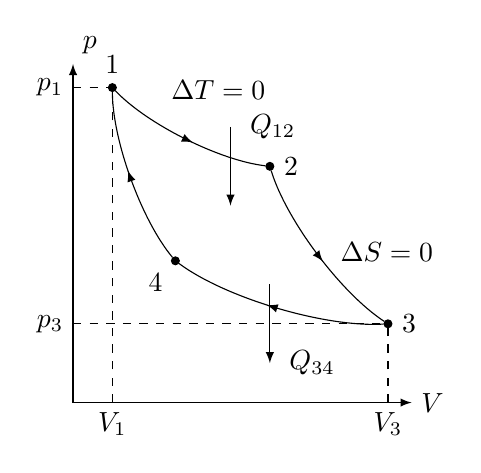
\begin{tikzpicture}[
  > = latex,
  dot/.style = {draw,fill,circle,inner sep=1pt},
  arrow inside/.style = {postaction=decorate,decoration={markings,mark=at position .55 with \arrow{>}}}
  ]
  \draw[<->] (0,4.3) node[above right] {$p$} |- (4.3,0) node[right] {$V$};
  \node[dot,label={above:$1$}] (@1) at (0.5,4) {};
  \node[dot,label={right:$2$}] (@2) at (2.5,3) {};
  \node[dot,label={right:$3$}] (@3) at (4,1) {};
  \node[dot,label={below left:$4$}] (@4) at (1.3,1.8) {};

  \node[label={above right:$\Delta T = 0$}] at (1,3.6) {};
  \node[label={above right:$\Delta S = 0$}] at (3.15,1.54) {};

  \draw[arrow inside] (@1) to[looseness=.7,bend right=20] (@2);
  \draw[arrow inside] (@2) to[looseness=.7,bend right=20] (@3);
  \draw[arrow inside] (@3) to[looseness=.7,bend left=20] (@4);
  \draw[arrow inside] (@4) to[looseness=.7,bend left=20] (@1);
  \draw[dashed,thin] (0,4) node[left] {$p_1$} -- (0.5,4);
  \draw[dashed,thin] (0,1) node[left] {$p_3$} -- (4,1);
  \draw[dashed,thin] (0.5,0) node[below] {$V_1$} -- (0.5,4);
  \draw[dashed,thin] (4,0) node[below] {$V_3$} -- (4,1);

  \draw[->] (2,3.5) to (2,2.5);
  \node[label={right:$Q_{12}$}] at (2,3.5) {};
  \draw[->] (2.5,1.5) to (2.5,0.5);
  \node[label={right:$Q_{34}$}] at (2.5,0.5) {};
\end{tikzpicture}

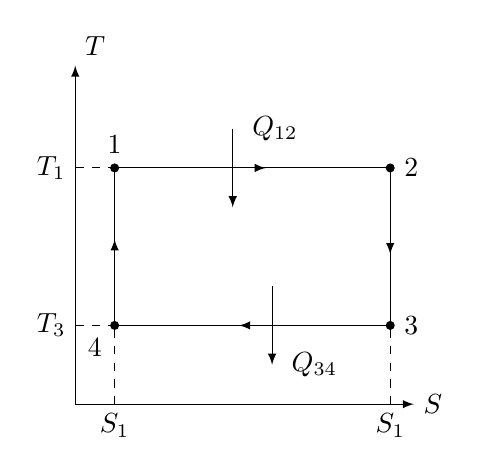
\begin{tikzpicture}[
  > = latex,
  dot/.style = {draw,fill,circle,inner sep=1pt},
  arrow inside/.style = {postaction=decorate,decoration={markings,mark=at position .55 with \arrow{>}}}
  ]
  \draw[<->] (0,4.3) node[above right] {$T$} |- (4.3,0) node[right] {$S$};
  \node[dot,label={above:$1$}] (@1) at (0.5,3) {};
  \node[dot,label={right:$2$}] (@2) at (4,3) {};
  \node[dot,label={right:$3$}] (@3) at (4,1) {};
  \node[dot,label={below left:$4$}] (@4) at (0.5,1) {};

  \draw[arrow inside] (@1) to (@2);
  \draw[arrow inside] (@2) to (@3);
  \draw[arrow inside] (@3) to (@4);
  \draw[arrow inside] (@4) to (@1);
  \draw[dashed,thin] (0,3) node[left] {$T_1$} -- (0.5,3);
  \draw[dashed,thin] (0,1) node[left] {$T_3$} -- (0.50,1);
  \draw[dashed,thin] (0.5,0) node[below] {$S_1$} -- (0.5,1);
  \draw[dashed,thin] (4,0) node[below] {$S_1$} -- (4,1);

  \draw[->] (2,3.5) to (2,2.5);
  \node[label={right:$Q_{12}$}] at (2,3.5) {};
  \draw[->] (2.5,1.5) to (2.5,0.5);
  \node[label={right:$Q_{34}$}] at (2.5,0.5) {};
\end{tikzpicture}

%   ______               _           __       
%  / ____/__  ____ ___  (_)_________/ /_  ___ 
% / / __/ _ \/ __ `__ \/ / ___/ ___/ __ \/ _ \
%/ /_/ /  __/ / / / / / (__  ) /__/ / / /  __/
%\____/\___/_/ /_/ /_/_/____/\___/_/ /_/\___/ 
%                                             
%    ____    __           __             ______              
%   /  _/___/ /__  ____ _/ /__  _____   / ____/___ _________ 
%   / // __  / _ \/ __ `/ / _ \/ ___/  / / __/ __ `/ ___/ _ \
% _/ // /_/ /  __/ /_/ / /  __/ /     / /_/ / /_/ (__  )  __/
%/___/\__,_/\___/\__,_/_/\___/_/      \____/\__,_/____/\___/ 
                                                            
\section{Gemische Idealer Gase}

\begin{align*}
	&\xi_i
	= \frac{m_i}{m}, \quad \psi_i
	= \frac{n_i}{n}, \quad p_i
	= \psi_ip \\
	&\xi_i
	= \frac{M_i n_i}{\sum_{k
	= 1}^{K} M_kn_k}
	= \frac{M_i}{M_G}\psi  
	\\
	& p_iV
	= m_iR_iT, \quad p_iV
	= n_iR_mT, \quad pV
	= mR_GT \\
	& \sum_{k
	= 1}^{K} p_k
	= p 
	\\
	&R_G
	= \frac{1}{m} \sum_{k=1}^{K} m_kR_k
	= \sum_{k=1}^{K} \xi_k R_k 
	\\
	&U_G
	= \sum_{k=1}^{K} U_k
	= \sum_{k=1}^{K} m_k u_k
	= \sum_{k=1}^{K} c_{vk}m_kT \leftarrow \text{$c_v$
	= const}
	\\
	&H_G
	= \sum_{k=1}^{K} H_k
	= \sum_{k=1}^{K} m_k h_k
	= \sum_{k=1}^{K} c_{pk}m_kT \leftarrow \text{$c_p$
	= const.}
	\\
	&c_{vG}
	= \sum_{k=1}^{K} c_{vk} \xi_k, \quad c_{pG}
	= \sum_{k=1}^{K} c_{pk}\xi_k 
	\\
	&S_2-S_1
	= R_m \left( n \ln n - \sum_{k=1}^{K} n_k \ln n_k \right)
\end{align*}

\begin{align*}
	\text{Adiabate } & \text{ Drosselung (ideal): } \\ 
	& h + \frac{c^2}{2} + gz = \text{const.} \\
	& dh = 0 \\
	\text{Adiabet } & \text{ Drosselung (real): }  \\ 
	& \delta_h = \left(\frac{\partial T}{\partial p}\right)_{h}  = - \frac{v}{c_p}(1-\beta T) \\
\end{align*}

%    _   __                    __                      ____
%   / | / /___ _______________/ /___ _____ ___  ____  / __/
%  /  |/ / __ `/ ___/ ___/ __  / __ `/ __ `__ \/ __ \/ /_  
% / /|  / /_/ (__  |__  ) /_/ / /_/ / / / / / / /_/ / __/  
%/_/ |_/\__,_/____/____/\__,_/\__,_/_/ /_/ /_/ .___/_/     
%                                           /_/            

\section{Nassdampf}
\tiny
\begin{flushleft}
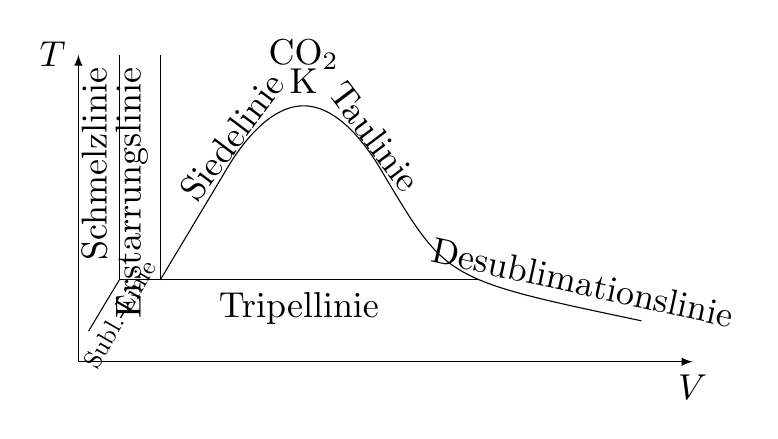
\begin{tikzpicture}
	[
	scale=1.3, every node/.style={scale=1.3},
	> = latex,
	dot/.style = {draw,fill,circle,inner sep=1pt},
	arrow inside/.style = {postaction=decorate,decoration={markings,mark=at position .55 with \arrow{>}}}
	]
	\draw[<->]  (0,3) node[left] {$T$} |- (6,0) node[below] {$V$} ;
	\draw (0.1,0.3) -- node[midway, below, rotate=60, scale=0.7] {Subl.-Linie} (0.4,0.8);
	\draw (0.4, 0.8) -- (0.4, 3) node[above left, rotate=90] {Schmelzlinie};
	\draw (0.8, 0.8) -- (0.8, 3) node[above left, rotate=90] {Erstarrungslinie};
	\draw (0.4,0.8) -- node[midway, below] {Tripellinie} (3.91,0.8);
	\draw (0.8,0.8) -- (1.4,1.8);
	\draw (1.4,1.8) parabola bend (2.2,2.5) (3,1.8);
	\draw (3,1.8)  .. controls (3.6,0.8) .. node[very near end, sloped, above] {Desublimationslinie} (5.5,0.4);
	\draw (1.5,2.2) node[rotate=53] {Siedelinie};
	\draw (2.9,2.2) node[rotate=-53] {Taulinie};
	\draw (2.2,3) node {$\text{CO}_\text{2}$};
	\draw (2.2,2.5) node[above] {K};
\end{tikzpicture}

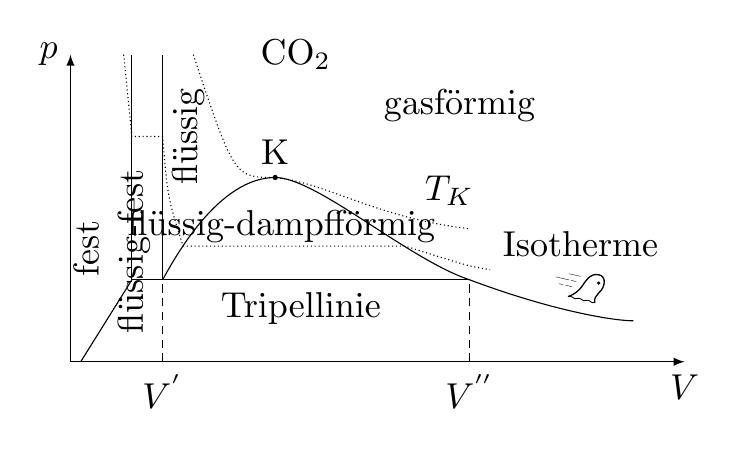
\begin{tikzpicture}
	[
	scale=1.3, every node/.style={scale=1.3},
	> = latex,
	dot/.style = {draw,fill,circle,inner sep=1pt},
	arrow inside/.style = {postaction=decorate,decoration={markings,mark=at position .55 with \arrow{>}}}
	]
	\draw[<->]  (0,3) node[left] {$p$} |- (6,0) node[below] {$V$} ;
	\draw (0.1,0) -- (0.6,0.8);
	\draw (0.6, 0.8) -- (0.6, 3) ;
	\draw (0.9, 0.8) -- (0.9, 3);
	\draw (0.6,0.8) -- node[midway, below] {Tripellinie} (3.9,0.8);

	\draw (0.9,0.8) parabola[bend at end]  (2, 1.8);

	\draw (2,1.8) .. controls (2.4,1.8) and (3.3, 1) .. (3.9,0.8) .. controls (4.7,0.5) and (5.3,0.4) .. node[above, sloped]  {$\xrightswishingghost{}$} (5.5,0.4);
	\draw (2.2,3) node {$\text{CO}_\text{2}$};

	\draw[fill] (2,1.8) circle (0.02) node[above] {K};

	\draw[densely dashed] (0.9,0) node[below] {$V^{'}$} -- (0.9,0.8);
	\draw[densely dashed] (3.9,0) node[below] {$V^{''}$} -- (3.9,0.8);
	\draw (3.7,1.4) node[above]  {$T_K$};
	\draw (0.4,1.5) node[above left, rotate=90] {fest};
	\draw (1.15,2.2) node[rotate=90] {flüssig};
 	\draw (0.9,2) node[above left, rotate=90] {flüssig-fest};
	\draw (2.06,1.32) node {flüssig-dampfförmig};
	\draw (3.8,2.5) node {gasförmig};

	\draw[densely dotted] (1.2,3) ..controls (1.6,1.8) .. (2,1.8) .. controls(2.5,1.75) and (3,1.4) .. (3.9, 1.3);
	\draw[densely dotted] (0.52,3) to (0.6,2.2) to (0.6,2.2) to (0.9,2.2) .. controls (0.95,1.6) .. (1.1,1.13) -- (3.27,1.13) .. controls (3.9,0.93) .. (4.1,0.9) node[above right] {Isotherme};
\end{tikzpicture}

%\small
%\begin{tikzpicture}
%	 [> = latex,
%	dot/.style = {draw,fill,circle,inner sep=1pt},
%	arrow inside/.style = {postaction=decorate,decoration={markings,mark=at position .55 with \arrow{>}}}
%	]
%	\draw[<->]  (0,3) node[left] {$p$} |- (3.5,0) node[below] {$v$};
%	\draw (1,1.8) parabola bend (1.5,2.4) (2,1.8);
%	\draw (0.4,0.3) -- (1,1.8);
%	\draw (2,1.8) to[bend right=10] (3,0.3);
%\end{tikzpicture}

\end{flushleft}
\normalsize
\begin{multicols}{2}

\begin{align*}
	& v = (1-x)v^{'} + xv{''} \\
	& v = v^{'} + (v^{''}-v^{'})x \\ \\
	& u = (1-x) u^{'} + xu^{''} \\
	& u = u^{'} + (u^{''}-u^{'})x \\ \\
	& h = (1-x) h^{'} + xh^{''} \\
	& h = h^{'} + (h^{''}-h^{'})x \\ \\
	& s = (1-x) s^{'} + xs^{''} \\
	& s = s^{'} + (s^{''}-s^{'})x \\ \\
	& r = h^{''} - h^{'} = T(s^{''}-s^{'}) \\
\end{align*}

\begin{align*}
	& T^{'} = T^{''} \\
	& p^{'} = p^{''} \\
	& g^{'} = g^{''} \\
	&dg^{'} = v^{'}dp^{'} - s^{'}dT^{'} \\
	&dg^{''} = v^{''} dp^{''} - s^{''} dT^{''} \\
	&dg^{'} = dg^{''} \\
	& \frac{dp}{dT} = \frac{s^{''} - s^{'}}{v^{''} - v^{'}} \\
	& \frac{dp}{dT} = \frac{1}{T}\frac{h^{''} - h^{'}}{v^{''} - v^{'}} \\
	& \frac{dp}{dT} = \frac{1}{T}\frac{r}{v^{''} -v^{'}} \\
\end{align*}
\end{multicols}

%    ____             __             _____ __        ________   _         
%   / __ \___  ____ _/ /__  _____   / ___// /_____  / __/ __/  (_)___ ___ 
%  / /_/ / _ \/ __ `/ / _ \/ ___/   \__ \/ __/ __ \/ /_/ /_   / / __ `__ \
% / _, _/  __/ /_/ / /  __/ /      ___/ / /_/ /_/ / __/ __/  / / / / / / /
%/_/ |_|\___/\__,_/_/\___/_/      /____/\__/\____/_/ /_/    /_/_/ /_/ /_/ 
%                                                                         
%    _   __                    __                      ____           __    _      __
%   / | / /___ _______________/ /___ _____ ___  ____  / __/___  ___  / /_  (_)__  / /
%  /  |/ / __ `/ ___/ ___/ __  / __ `/ __ `__ \/ __ \/ /_/ __ `/ _ \/ __ \/ / _ \/ _/
% / /|  / /_/ (__  |__  ) /_/ / /_/ / / / / / / /_/ / __/ /_/ /  __/ /_/ / /  __/ /__
%/_/ |_/\__,_/____/____/\__,_/\__,_/_/ /_/ /_/ .___/_/  \__, /\___/_.___/_/\ __/\___/
%                                           /_/        /____/                 

\section{Realer Stoff im Nassdampfgebiet}
\begin{align*}
	\text{Isobare } &\text{Zustandsänderung} \\
	&q_{12} = T(s_2 - s_1) = T\Big(s^{''} - s^{'}\Big)(x_2-x_1) \\
	&w_{V,12} = - \int_{1}^{2} p\; dv = -p(v_2-v_1) = -p\Big(v^{''} -v^{'}\Big)(x_2-x_1) \\
	\text{Isochore } &\text{Zustandsänderung} \\
	&q_{12} = u_2 - u_1 = u_2^{'} + x_2\Big(u_2^{''} - u_2^{'} \Big) - u_1^{'} - x_1\Big(u_1^{''} - u_1^{'}\Big) \\
	\text{Adiabate } &\text{Zustandsänderung} \\
	& w_{V,12} = u_2 - u_1 = u_2^{'} + x_2 \Big( u_2^{''} - u_2^{'} \Big) - u_1^{'} - x_1\Big(u_1^{''} - u_1^{'}\Big) \\
\end{align*}

Entropieänderung wärend des Mischvorgangs
\begin{equation*}
	S_2-S_2 = R_m \left ( n \ln n - \sum_{i}^{} n_i \ln n_i \right )
\end{equation*}
\pagebreak

%    ______                     _    
%   / ____/  _____  _________ _(_)__ 
%  / __/ | |/_/ _ \/ ___/ __ `/ / _ \
% / /____>  </  __/ /  / /_/ / /  __/
%/_____/_/|_|\___/_/   \__, /_/\___/ 
%	              /____/         

\section{Maximale Arbeit und Exergie}
%Die Exergie ist die maximal nutzbare Arbeit eines Systms, dass von seinem ursprünglichen Zustand, isentrop und reibungsfrei, in den Umgebungszustand überführt wird.
Maxiaml nutzbare Arbeit $\rightarrow$ isentrop, reibungsfrei \\
%Man bewegt sich erst isentrop auf die isotherme der Umgebungsthemperatur und führt dann isotherm Wärem zu/ab, bis man den Umgebungszustand erreicht hat. 
$1 \rightarrow 1'$ : isentrop auf $T_u$ \\
$1' \rightarrow u$ : isotherm auf $u$ 

\begin{multicols}{2}


	\begin{flushleft}

\begin{tikzpicture}[
	scale=0.8, every node/.style={scale=1},
  > = latex,
  dot/.style = {draw,fill,circle,inner sep=1pt},
  arrow inside/.style = {postaction=decorate,decoration={markings,mark=at position .55 with \arrow{>}}}
  ]
  	\draw[<->] (0,4.3) node[above right] {$T$} |- (4.3,0) node[right] {$S$};

	\coordinate (a) at (0.8,0.6);
	\coordinate (b) at (0.8,2);

	\coordinate (c) at (3.3,3.5);
	\coordinate (d) at (3.3,2);

	\coordinate (u) at (2,2);
	\node[dot,label={above left:$u$}] at (u) {};

	\node[dot,label={below left:$1$}] at (a) {};
	\node[dot,label={above left:$1'$}] at (b) {};

  	\draw[thick, arrow inside] (a) to (b);
  	\draw[thick, arrow inside] (b) to (u);

	\node[dot,label={below left:$2$}] at (c) {};
	\node[dot,label={above left:$2'$}] at (d) {};

  	\draw[thick, arrow inside] (c) to (d);
  	\draw[thick, arrow inside] (d) to (u);

  	\draw[dashed,thin] (0,2) node[left] {$T_u$} -- (2,2);
  	\draw[dashed,thin] (2,0) node[below] {$S_u$} -- (2,2);

\end{tikzpicture}
\end{flushleft}
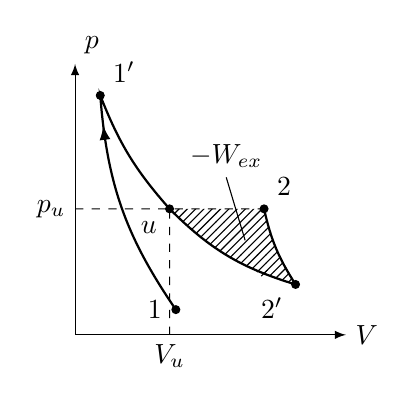
\begin{tikzpicture}[
	scale=0.8, every node/.style={scale=1},
  > = latex,
  dot/.style = {draw,fill,circle,inner sep=1pt},
  arrow inside/.style = {postaction=decorate,decoration={markings,mark=at position .55 with \arrow{>}}}
  ]
  \draw[<->] (0,4.3) node[above right] {$p$} |- (4.3,0) node[right] {$V$};
	\coordinate (a) at (1.6,0.4);
	\coordinate (b) at (0.4,3.8);

	\coordinate (c) at (3,2);
	\coordinate (d) at (3.5,0.8);

	\coordinate (u) at (1.5,2);
	\node[dot,label={below left:$u$}] at (u) {};

	\node[dot,label={left:$1$}] at (a) {};
	\node[dot,label={above right:$1'$}] at (b) {};

	\draw[thick, arrow inside] (a) to[bend left=15] (b) to[bend right=10] (u);

	\node[dot,label={above right:$2$}] at (c) {};
	\node[dot,label={below left:$2'$}] at (d) {};

	\draw[thick, arrow inside, pattern=north east lines] (c) to[bend right=10] (d) to[bend left=14] (u);
	\draw (2.7,1.5) to (2.4,2.5) node[above] {$-W_{ex}$};

  	\draw[dashed,thin] (0,2) node[left] {$p_u$} -- (c);
  	\draw[dashed,thin] (1.5,0) node[below] {$V_u$} -- (u);
\end{tikzpicture}
\end{multicols}

\begin{multline*}
	-\dot{W}_{ex} = - (\dot{W}_t)_{rev} = -\frac{d}{dt} \left( U + m\left ( \frac{c^2}{2}+ gz \right) + p_uV - T_uS \right) \\  +  \sum_{j=1}^{K} \left(\dot{m}_j \left(h + \frac{c^2}{2} + gz -T_s \right) \right) + \sum_{l=1}^{K} \left( 1 - \frac{T_u}{T}\right) \dot{Q}_l 
\end{multline*}


Die Exergie der Enthalpie (offens, stationäres System)
\begin{equation*}
	-\dot{W}_{ex,1u} = \dot{m}(h_1 - h_u -T_u(s_1 - s_u))
\end{equation*}
Die Exergie der inneren Energie (geschlossenes, instationäres System)
\begin{align*}
	- \dot{W}_{ex} &= - \frac{d}{dt}(U + p_uV -T_uS) \\
	-\dot{W}_{ex,1u} &= U_1 - U_u -p_u(V_1 - V_u) - T_u(S_1 - S_u)
\end{align*}
Für Ideales Gas \\
\begin{align*}
	-W_{ex} = mc_v(T_1 -T_u) + p_u(V_1 - V_u) - T_um \left(c_p \ln \left(\frac{T_1}{T_u}\right) -R_i \ln \left(\frac{p_1}{p_u}\right)\right)
\end{align*}
Dampf/Luftdruckkammer
\begin{equation*}
	-W_{ex,1u} = m_1 [ u_1 - u_u + p_u ( v_1 - v_u) - T_u(s_1 - s_u)]
\end{equation*}
Die Exergie der Wärme (geschlossenes, stationäres System)
\begin{equation*}
	- \dot{W}_{ex} = \left(1 - \frac{T_u}{T_1} \right) \dot{Q}_1 = \eta_{th,C} \dot{Q}_1 \\
\end{equation*}
\pagebreak

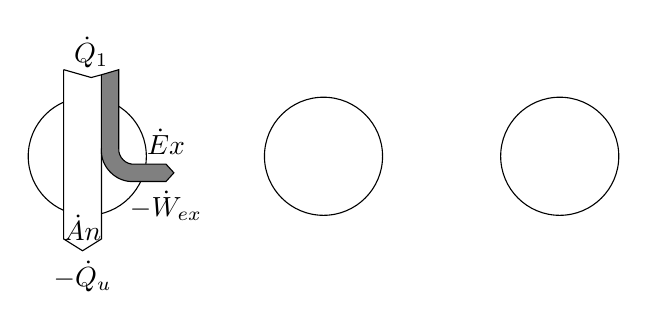
\begin{tikzpicture}[
		\thicc
		]
	\coordinate (a1) at (0.7,2.3);
	\coordinate (a2) at (1.05,2.2);
	\coordinate (a3) at (1.18,2.235);
	\coordinate (a4) at (1.18,0.15);
	\coordinate (a5) at (0.94,0);
	\coordinate (a6) at (0.7,0.15);
	\coordinate (a7) at (1.4,2.3);
	\coordinate (a8) at (1.4,1.3);
	\coordinate (a9) at (1.6,1.1);
	\coordinate (a10) at (2,1.1);
	\coordinate (a11) at (2.1,0.99);
	\coordinate (a12) at (2,0.88);
	\coordinate (a13) at (1.6,0.88);
	\coordinate (a14) at (1.18,1.3);
	
	\draw 	(1,1.2) node [minimum size=1.5cm,circle,draw] {};
	\draw[fill=white] 	(a1) to (a2) to (a3) to (a4) to (a5) to (a6) to (a1);
	\draw[fill=gray] 	(a3) to (a7) to (a8) to[bend right=50] (a9) to (a10) to (a11) to (a12) to (a13) to[bend left=50] (a14);
	\draw (a3) to (a4);
	\draw 	(4,1.2) node [minimum size=1.5cm,circle,draw] {};
	\draw 	(7,1.2) node [minimum size=1.5cm,circle,draw] {};

	\draw 	(a2) node[above] {$\dot{Q}_1$};
	\draw 	(a5) node[above] {$\dot{A}n$};
	\draw 	(a5) node[below] {$-\dot{Q}_u$};
	\draw 	(a10) node[above] {$\dot{E}x$};
	\draw 	(a12) node[below] {$-\dot{W}_{ex}$};
\end{tikzpicture}

                   
% _       __ /\// /|___/|                   __                           _ __   /\// /|___/|_ 
%| |     / ///\/ | __  /________ ___  ___  / /______ _____  ____ _____  (_) /__//\/ | __  / /_
%| | /| / / _ | / /_/ / ___/ __ `__ \/ _ \/ //_/ __ `/ __ \/ __ `/_  / / / __/ _ | / /_/ / __/
%| |/ |/ / __ |/___  / /  / / / / / /  __/ ,< / /_/ / /_/ / /_/ / / /_/ / /_/ __ |/___  / /_  
%|__/|__/_/ |_|/   |/_/  /_/ /_/ /_/\___/_/|_|\__,_/ .___/\__,_/ /___/_/\__/_/ |_|/   |/\__/  
%                                                 /_/                                         
\section{Wärmekapazität}

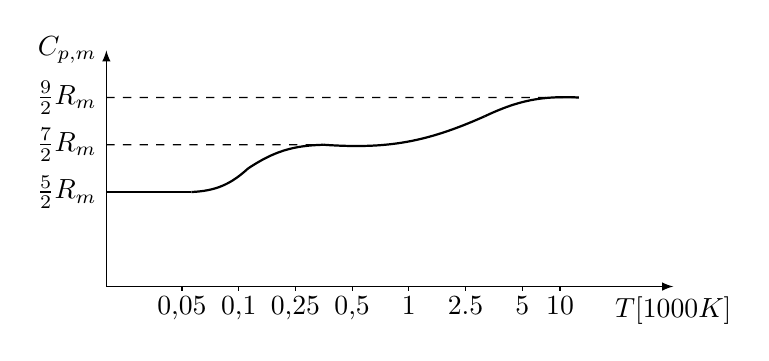
\begin{tikzpicture}[
	scale=1.2, every node/.style={scale=1},
  > = latex,
  dot/.style = {draw,fill,circle,inner sep=1pt},
  arrow inside/.style = {postaction=decorate,decoration={markings,mark=at position .55 with \arrow{>}}}
  ]
	\draw[<->] (0,2.5) node[left] {$C_{p,m}$} |- (6,0) node[below] {$T[1000K]$};

	\coordinate (a) at (0,1);
	\coordinate (b) at (0.9,1);
	\coordinate (c) at (1.5,1.25);
	\coordinate (d) at (2.3,1.5);
	\coordinate (e) at (4,1.8);
	\coordinate (f) at (5,2);
	
	\coordinate (g) at (0.8,0);
	\coordinate (h) at (1.4,0);
	\coordinate (i) at (2.0,0);
	\coordinate (j) at (2.6,0);
	\coordinate (k) at (3.2,0);
	\coordinate (l) at (3.8,0);
	\coordinate (m) at (4.4,0);
	\coordinate (n) at (4.8,0);

	\draw[dashed] (0,2) node[left] {$\frac{9}{2}R_m$} -- (f);
	\draw[dashed] (0,1.5) node[left] {$\frac{7}{2}R_m$} -- (d);
	\draw (a) node[left] {$\frac{5}{2}R_m$};

	\draw[thick] (a) to (b);
	\draw[thick] (b) to[bend right=20] (c);
	\draw[thick] (c) to[bend left=16] (d);
	\draw[thick] (d) to[bend right=14] (e);
	\draw[thick] (e) to[bend left=14] (f);

	\draw (g) node[below] {0,05} to ($ (g) - (0,0.05) $);
	\draw (h) node[below] {0,1} to ($ (h) - (0,0.05) $);
	\draw (i) node[below] {0,25} to ($ (i) - (0,0.05) $);
	\draw (j) node[below] {0,5} to ($ (j) - (0,0.05) $);
	\draw (k) node[below] {1} to ($ (k) - (0,0.05) $);
	\draw (l) node[below] {2.5} to ($ (l) - (0,0.05) $);
	\draw (m) node[below] {5} to ($ (m) - (0,0.05) $);
	\draw (n) node[below] {10} to ($ (n) - (0,0.05) $);
\end{tikzpicture}

\begin{align*}
	&	C_{v,m} = \frac{1}{\kappa - 1} R_m,
	\quad	C_{p,m} = \frac{\kappa}{\kappa -1}r_m \\
	&	c_v = \frac{1}{\kappa - 1 }R_j, 
	\qquad	c_p = \frac{\kappa}{\kappa -1}R_j \\
	&	\kappa = \frac{c_p}{c_v},
	\qquad \qquad \; \:   c_p - c_v = R\\
	\end{align*}
	\begin{multline*}
		C_{v,m} = \underbrace{3 + \frac{R_m}{2}}_{\text{Translatorisch}} + \underbrace{\frac{n_{\text{rot}}  R_m}{2}}_{\text{Rotatorisch}}  
		+ \underbrace{R_M ( 3n_{\text{Atome}} - 3 - n_{rot})}_{\text{Vibratorisch}}  \\
		+ \underbrace{C_{v,m,Elektronenanregung}}_{\text{Relevant ab: }T \approx 10^4K } 
	\end{multline*}

\onecolumn

%       ____    __           __             ______              
%      /  _/___/ /__  ____ _/ /__  _____   / ____/___ ______    
%      / // __  / _ \/ __ `/ / _ \/ ___/  / / __/ __ `/ ___/    
%    _/ // /_/ /  __/ /_/ / /  __(__  )  / /_/ / /_/ (__  )     
%   /___/\__,_/\___/\__,_/_/\___/____/   \____/\__,_/____/      
                                                               
\begin{landscape}
	\LARGE
	Ideales Gas 
	\\\\
	\renewcommand{\arraystretch}{2}
\begin{tabular}{l|l|l|l|l|l}
& Isothermo  
& Isobare  
& Isochore  
& Isentrop  
& Polytrope 
\\ \hline
  konstant:  
& T  
& p  
& v  
& $\delta q=0$  
& $pv^n$  
\\ \hline
	
& -  
& -  
& -  
& $p_1 v_1^{\kappa} = p_2 v_2^{\kappa}$  
& $v_1^{n} = p_2 v_2^{n}$  
\\ \hline

& $p_1 p_2 = p_2 v_2$  
& $\frac{v_1}{v_2} = \frac{T_1}{T_2}$  
& $\frac{p_1}{T_1} = \frac{p_2}{T_2}$  
& $T_1 v_1^{\kappa - 1} = T_2 v_2^{\kappa -1}$   
& $T_1 v_1^{n - 1} = T_2 v_2^{n -1}$  
\\ \hline
	
& -  
& -  
& $\small\xrightswishingghost{}$  
& $\frac{T_1^{\frac{\kappa}{\kappa -1}}}{p_1} = \frac{T_2^{\frac{\kappa}{\kappa -1}}}{p_2}$  
& $\frac{T_1^{\frac{n}{n -1}}}{p_1} = \frac{T_2^{\frac{n}{n -1}}}{p_2}$  
\\ \hline

	$p,v$

& $p = \frac{p_1 v_1}{v}$  
& $p = p_1$  
& $v = v_1$  
& $p = \frac{p_1 v_1^{\kappa}}{v^{\kappa}}$  
& $p = \frac{p_1 v_1^{n}}{v^{n}}$ 
\\ \hline

	$p,T$

& $p = \frac{p_1 v_1}{v}$  
& $p = p_1$  
& $p = \frac{p_1}{T_1}T$  
& $p = \frac{p_1}{T_1^{\frac{\kappa}{\kappa -1}}} T^{\frac{\kappa}{\kappa -1}}$  
& $p = \frac{p_1}{T_1^{\frac{n}{n -1}}} T^{\frac{n}{n -1}}$
\\ \hline

	$v,T$  

& $T = T_1$  
& $v = \frac{v_1}{T_1}T$  
& $v = v_1 $ 
& $T = \frac{T_1 v_1^{\kappa - 1}}{v^{\kappa - 1}}$  
& $T = \frac{T_1v_1^{n-1}}{v^{n-1}}  $
\\ \hline

	$q_{12}$	

& $= p_1v_1 \ln \frac{p_1}{p_2}$  
& $= c_p(T_2 - T_1)$   
& $= c_v(T_2 - T_1)$  
& $= 0$   
&  $= c_v \frac{n-\kappa}{n-1}(T_2-T_1)$ 
\\ \hline

	$w_{V,12}$  

& $= -q_{12}$ 
& $= -p_1(v_2 - v_1)$  
& $= 0$  
& $= \frac{p_1 v_1}{k - 1}\left[\left(\frac{v_1}{v_1}\right)^{\kappa - 1} - 1\right]$  
& $= \frac{p_1 v_1}{n - 1}\left[\left(\frac{v_1}{v_2}\right)^{n-1} - 1\right]$ 
\\ \hline

	$s_2 - s_1$ 

& $s_2 -s_1 = R \ln \left(\frac{p_1}{p_2}\right)$  
& $= c_p \ln \left(\frac{T_2}{T_1}\right)$  
& $= c_v \ln \left(\frac{T_2}{T_1}\right)$  
& $= 0$  
& $= c_v \frac{n - \kappa }{n - 1} \ln \left(\frac{T_2}{T_1}\right)$  
\\ 
\end{tabular}
\bigskip
\\\\
% _    __                  ____                _       __            __         
%| |  / /___ _____        / __ \___  _____    | |     / /___ _____ _/ /____     
%| | / / __ `/ __ \______/ / / / _ \/ ___/____| | /| / / __ `/ __ `/ / ___/_____
%| |/ / /_/ / / / /_____/ /_/ /  __/ /  /_____/ |/ |/ / /_/ / /_/ / (__  )_____/
%|___/\__,_/_/ /_/     /_____/\___/_/         |__/|__/\__,_/\__,_/_/____/       
%                                                                               
%   ______                
%  / ____/___ ______      
% / / __/ __ `/ ___/      
%/ /_/ / /_/ (__  )       
%\____/\__,_/____/        

\Large
Van-Der-Waals-Gas  
\\

	\begin{tabular}{l|l|l|l|l}
		
& Isotherme 
& Isobare 
& Isochore 
& Isentrop 
\\ \hline
		konst. 
& T 
& p 
& v  
& $\delta = 0$ 
\\ \hline
		
& \thead{\Large$(p_1 + \frac{a}{v^2})(v_1-b)$ \\\Large $= (p_2 + \frac{a}{v^2})(v_2-b)$}
& \Large$\frac{RT_1}{v_1-b} - \frac{a}{v_1^2} = \frac{RT_2}{v-b} - \frac{a}{v_2^2}$ 
& $\frac{p_1 + \frac{a}{v_1^2}}{T_1} = \frac{p_2 + \frac{a}{v_1^2}}{T_2}$  
& \thead{\large $(p_1 + \frac{a}{v^2}) (v_1-b)^{\frac{c_v + R}{c_v}}$ \\\large $ = (p + \frac{a}{v^2}) (v_2-b)^{\frac{c_v + R}{c_v}},$ \\ \large $ \quad T_1(v_1-b)^{R/c_v} = T_2 (v_2-b)^{R/c_v}$}  
\\ \hline

		$p,v$ 

& $p = (p + \frac{a}{v^2}) \frac{v_u}{v-b} - \frac{a}{v^2}$ 
& $p = p_1$  
& $v = v_1$ 
& $p = - \frac{a}{v^2} + (p_1 + \frac{a}{v^2}) \left(\frac{v_1-b}{v_m}\right)^{\frac{v_v + R }{R}}$ 
\\ \hline

		$p,T$ 

& $T = T_1$ 
& $p = p_1$ 
& $p = \frac{T}{T_1} (p_1 + \frac{a}{v^2}) - \frac{a}{v_1^2}$ 
& $p = - \frac{a}{v^2}+ (p_1 + \frac{a}{v^2}) \left(\frac{T}{T_1}\right)^\frac{c_v+R}{R}$ 
\\ \hline

		$v,T$ 

& $T = T_1$ 
& $T = T_1 \frac{v-b}{v_1-b} + \frac{a}{R}(v-b) \left(\frac{1}{v^2} - \frac{1}{v_1^2}\right)$ 
& $v = v_1$  
& $T = T_1 \left(\frac{v_1-b}{v-b}\right)^\frac{R}{c_v}$ 
\\ \hline

		$q_{12}$ 

& $= RT_1 \ln \left(\frac{v_2-b}{v_1-b}\right)$ 
& $= \frac{a}{v_1} - \frac{a}{v_2} + c_v(T_2 - T_1) + p_1(v_2 - v_1)$ 
& $= c_v(T_2 - T_1)$  
& $= 0$  
\\ \hline

		$w_{V,12}$ 

& $= -RT_1 \ln \left(\frac{v_2-b}{v_1-b}\right) + \frac{a}{v_1} - \frac{a}{v_2}$ 
& $= -p_1(v_2-v_1)$ 
& $= 0$  
& $= \frac{a}{v_1} - \frac{a}{v_2} + c_v(T_2 - T_1)$ 
\\ \hline

		$s_2 - s_1$ 

& $= R\ln \left(\frac{v_2-b}{v_1-b}\right)$ 
& $= c_v \ln \left(\frac{T_2}{T_1}\right) + R \ln \left(\frac{v_2-b}{v_1-b}\right)$ 
& $= c_v \ln \left(\frac{T_2}{T_1}\right)$ 
& $= 0$ 
\\
\end{tabular}

\end{landscape}

\end{document}

